\documentclass[a4paper,11pt]{article}

% set up sensible margins (same as for cssethesis)
\usepackage[paper=a4paper,left=30mm,right=30mm,top=25mm,bottom=25mm]{geometry}
\usepackage{natbib} % Use the natbib bibliography and citation package
\usepackage{setspace} % This is used in the title page
\usepackage{graphicx} % This is used to load the crest in the title page

% non-template packages
\usepackage{paralist}
\usepackage{multicol}
\usepackage{caption}
\usepackage{tabularx, booktabs}
\newcolumntype{Y}{>{\centering\arraybackslash}X}


\usepackage{hyperref}
\usepackage{xcolor}
\usepackage{lscape}
\hypersetup{
	colorlinks,
	linkcolor=teal,
	citecolor=teal,
	urlcolor=blue
}

%tikz stuff
\usepackage{tikz}
\usetikzlibrary{shapes, arrows, trees}
\tikzstyle{decision} = [diamond, draw, fill=green!20, text width=4.5em, text badly centered, node distance=3cm, inner sep=0pt]
\tikzstyle{block} = [rectangle, draw, fill=yellow!20, text width=3cm, text centered, rounded corners, minimum height=4em]
\tikzstyle{line} = [draw, -latex']
\tikzstyle{straight} = [draw]


\usepackage{array}
\newcolumntype{L}[1]{>{\raggedright\let\newline\\\arraybackslash\hspace{0pt}}m{#1}}
\newcolumntype{C}[1]{>{\centering\let\newline\\\arraybackslash\hspace{0pt}}m{#1}}
\newcolumntype{R}[1]{>{\raggedleft\let\newline\\\arraybackslash\hspace{0pt}}m{#1}}


%\hypersetup{
%	colorlinks,
%	linkcolor={red!50!black},
%	citecolor={blue!50!black},
%	urlcolor={blue!80!black}
%}

\begin{document}

% Set up a title page
\thispagestyle{empty} % no page number on very first page
% Use roman numerals for page numbers initially
\renewcommand{\thepage}{\roman{page}}

\begin{spacing}{1.5}
\begin{center}
{\Large \bfseries
School of Computer Science \\
Monash University}

\vspace*{30mm}


\includegraphics[width=5cm]{graphics/MonashCrest.pdf}

\vspace*{15mm}

{\large \bfseries
Research Proposal --- Comp Sci Honours, 2017
}

\vspace*{10mm}

{\LARGE \bfseries
Exploring improvements to Part-to-picker systems in Warehouses 
}

\vspace*{20mm}

{\large \bfseries
Phillip Wong 25150510

\vspace*{20mm}


%Supervisors: \parbox[t]{50mm}{Daniel Harabor}, \\Another person}
Supervisor: Daniel Harabor
}

\end{center}
\end{spacing}

\newpage

\tableofcontents

\newpage
% Now reset page number counter,and switch to arabic numerals for remaining
% page numbers 
\setcounter{page}{1}
\renewcommand{\thepage}{\arabic{page}}

	\begin{abstract} %100-200 words
	\noindent \textbf The order picking process is the number one expense in warehouse systems. Here we look at part-to-picker a type of order picking where the products are autonomously retrieved and given to the pickers. Previous research have focused on improvements in the multi-agent path finding but they often overlook simple adjustments or additions which may help improve the overall complexity of the problem. This project will test the effect that these [\textbf{LIST THINGS}] have on improving order-picking. We will create a simulation and focus on the warehouse layout first. The results of this project will help identify how small adjustments may affect the efficiency of the order picking process.
	
\end{abstract}
\section{Introduction}
Order picking is a process in warehouse systems whereby a product is retrieved according an incoming customer order. This process has been identified by \cite{de2007design} as the most costly process in operating a warehouse, estimated to take 55\% of the warehouse operating cost.


Here we look at a method of order picking known as part-to-picker systems which automates the movement of products from where they are stored to a picking stations, where workers will manually pick the orders. (\cite{wurman2008coordinating}). Part-to-picker systems often employ the use of automated vehicles when retrieve the orders from where they are stored. \cite{introduction2015autostore} is a recent system where products are organized in a grid of stacked bins. Robots move around the top of the grid, lifting bins and delivering them to a human picker. Benefits of the AutoStore system include high storage density and expansion capability. While not much literature is published about the specifics of AutoStore, we suspect some downsides of this system to be similar to conveyor belts with high operational and maintenance costs as well as high retrieval cost.

In this project we look at Kiva Systems (now known as Amazon Robotics). In Kiva systems, products are stored in shelves known as storage pods. Robots known as drive units are responsible for picking up and carrying storage pods to picking stations (see Fig \ref{kivaprocess} and \ref{kivalayout1}).
\begin{figure}[h!]
	\centering
	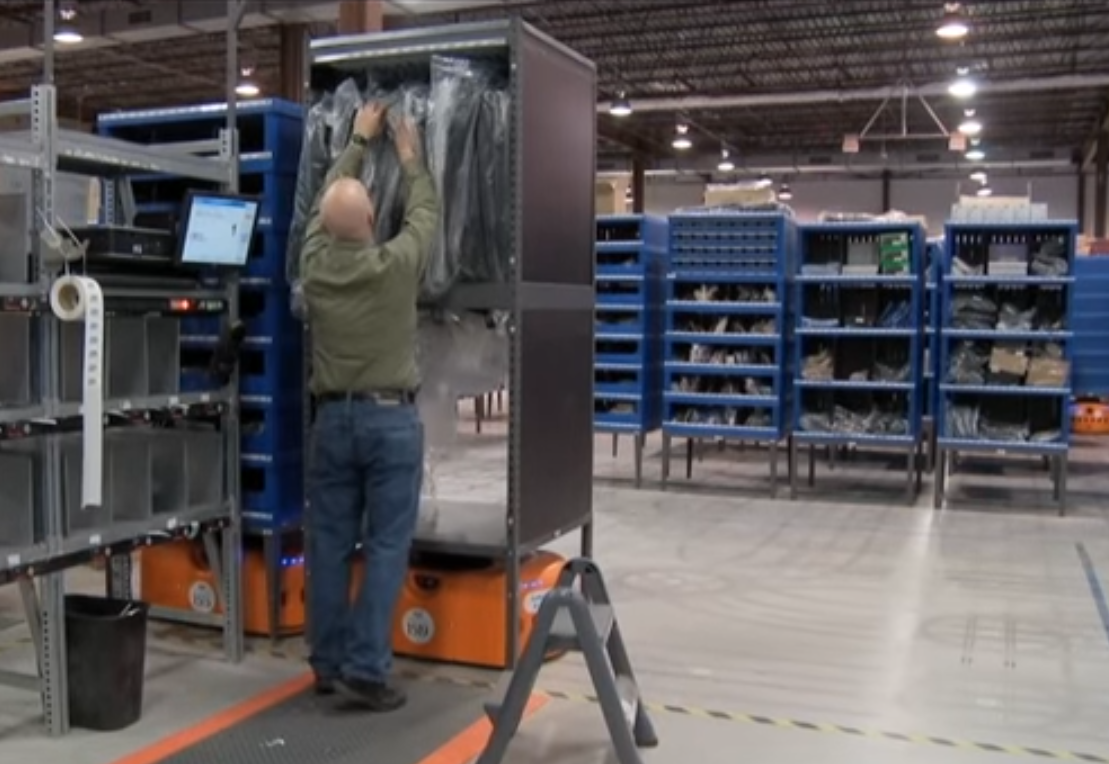
\includegraphics[width=0.8\textwidth ]{graphics/kivaprocess}
	\caption{A worker picking an order from a storage pod. The orange robot underneath is the drive unit. (\cite{kivayoutube2010quietlogistics})}
	\label{kivaprocess}
\end{figure}

\noindent The process for a drive unit is as follows:

\begin{compactenum}
	\item Unit is told to retrieve a product
	\item Unit moves to the storage pod containing the product and picks up the pod
	\item Unit carries the pod to a picking station
	\item Human worker picks the product from the pod and packs it
	\item Unit returns the pod back to where it was picked up
	\item Unit waits until it is told to retrieve another product
\end{compactenum}

\noindent Kiva systems do not require a complex infrastructure to operate hence solving issues found in alternative solutions: maintenance and operational costs. When a unit malfunctions it can be easily accessed and replaced, moreover the system remains operational. The initial setup for a warehouse is cheap and fast as a warehouse needs only storage pods, a picking station and a number of drive units to operate.

\subsection{Research questions}
In order to explore the improvements that can be made to improving Kiva systems, we aim to answer two main questions:

\begin{enumerate}
	\item What adjustments can be made to Kiva systems to simplify the pathfinding?
\begin{compactitem}
	\item An improved layout of storage pods and picking stations
	\item Allowing drive units are capable of maneuvering underneath storage pods
	\item An intermediate zone for drive units to drop off storage pods
\end{compactitem}

\item How much faster will the path search run by pre-computing paths and storing them in a path oracle?

\end{enumerate}

\section{Background}
\label{background}
% Description of MAPF problem, including objective function

Kiva Systems deal with a number of problems, in this project we will be focusing on the multi-agent pathfinding (MAPF) problem. MAPF aims to find a path from for each agent so that they can reach their goal while ensuring that no path conflicts with another, in our case an agent is a drive unit and the goal is either a storage pod or picking station. When analyzing the performance of a MAPF solution we generally look at the makespan of the system. In our case of Kiva systems we will also be looking at the downtime of picking stations. Outside of order picking and warehouse applications,  MAPF has usage in video games, robotics (\cite{bennewitz2002finding}), search and rescue (\cite{konolige2006centibots}) and automated ports.

% How hard is it?
Finding an optimal solution to multi-agent pathfinding is an NP-hard problem (\cite{yu2013structure}), has applications in systems containing few agents. This is not an option as Kiva systems deal with hundreds of agents, for example the Office Supply company, Staples uses 500 robots in their 30000$m^{2}$ center (\cite{guizzo2008three}). At the current time, the best we can get is a bounded suboptimal solution and this has been explored by a number of existing literature (\cite{cohen2016bounded}).

% What are the main way people solve it?
Generally methods are provided to simplify the MAPF problem, \cite{cohen2016bounded} uses user-provided highways which guide agents towards a specific direction. \cite{wilt2014spatially} identifies bottlenecks in the environment and creates a controller which handles the agents who want to pass through the bottleneck. Another common simplification is grouping agents into teams. \cite{ma2016optimal} splits agents into teams of 5 and presents a Conflict-Based Min-Cost-Flow algorithm which and shows that they can achieve a correct, complete and optimal solution. \textbf{I'm not sure what the downside of this is...besides the fact that you generalize agents into teams of 5}.

% What are the main advantages and drawbacks of each approach?


%\cite{de2007design} provides a great overview of picking
Specific to order picking, it is possible to assist MAPF by manipulated incoming orders to suit the location of products. For example if a large order of one product came in, this could be interlaced with other orders, so agents do not need to all head to the same location. In a similar fashion, MAPF can be assisted by smart distribution of products across the warehouse. Take the same example where a large order of one product comes in, if the products were spread out around the warehouse and not situated next to one another this would not be an issue. This method is especially relevant in Kiva systems as storage pods can be easily moved around the warehouse by the drive units. \cite{boysen2017parts} looks at both of these aspects and found that with optimized order processing, only half the units are required to provide the supply given by a non-optimized system.

%\cite{wurman2008coordinating} provides an in depth overview of Kiva Systems, describing their benefits, usages and research areas.

%\cite{gu2010research} provides a comprehensive review of warehouse design and performance. It covers 5 major aspects, overall structure, sizing and dimensioning, department layout, equipment selection and operation strategy selection.

%\cite{de2007design} provides a survey on order picking

%\cite{strasser2015compressing} uses Compressed Path Databases.

%Unlike existing literature, in this project we aim looking at a number of other factors which are likely to simplify the pathfinding problem.

%Windowed Hierarchical Cooperative A∗. Cooperative A*. Conflict-Oriented Windowed Hierarchical Cooperative A∗. Compressed Path Databases.

\section{Methodology}
\label{Research}
\subsection{Path oracle}

Decentralised approaches are usually used in MAPF algorithms due to their lower CPU and memory requirements (\cite{wang2009bridging}) compared to a centralised approach. Decentralised MAPF involves agents independently searching for a path to their goal. Once a path is found, agents take turns follow their path one step at a time until a collision occurs between some agents. We favor an agent based on some utility function and the other agent will wait or find a new path. Hence computing paths becomes very costly as we increase the number of agents and consequently the number of path collisions. Here aim to introduce a path oracle which will pre-compute paths, removing the need for agents to perform a search at runtime. We expect to base this off the work by \cite{strasser2015compressing}, utilizing a Compressed Path Database.

%\noindent \textbf{PLACEHOLDER} Decentralised MAPF algorithms usually involve search. A typical problem solving process (e.g. FAR (Wang \& Botea, ICAPS 2008)) involves each agent finding a path independent from all the rest (i.e. if there are k agents we solve k single-agent problems separately). When all agents have a path they each take turns moving one step at a time towards their goal. Conflicts are resolved locally choosing in favour of one agent over another in some way (e.g. assign a priority to each agent and always favour the agent with highest priority). We aim to improve efficiency by introducing a path oracle which removes entirely the need to search. The oracle is pre-computed up front and reused for every subsequent pathfinding query thereafter. Since the cost of the initial path searches tends to dominate runtime in MAPF we expect this approach will significantly improve performance. \textbf{PLACEHOLDER}

\subsection{Warehouse layout}
\label{warehouselayout}
Usually the picking station is positioned on one side of the warehouse and the pods are laid out in rows (Fig. \ref{kivalayout1}).

\begin{figure}[h]
	\centering
	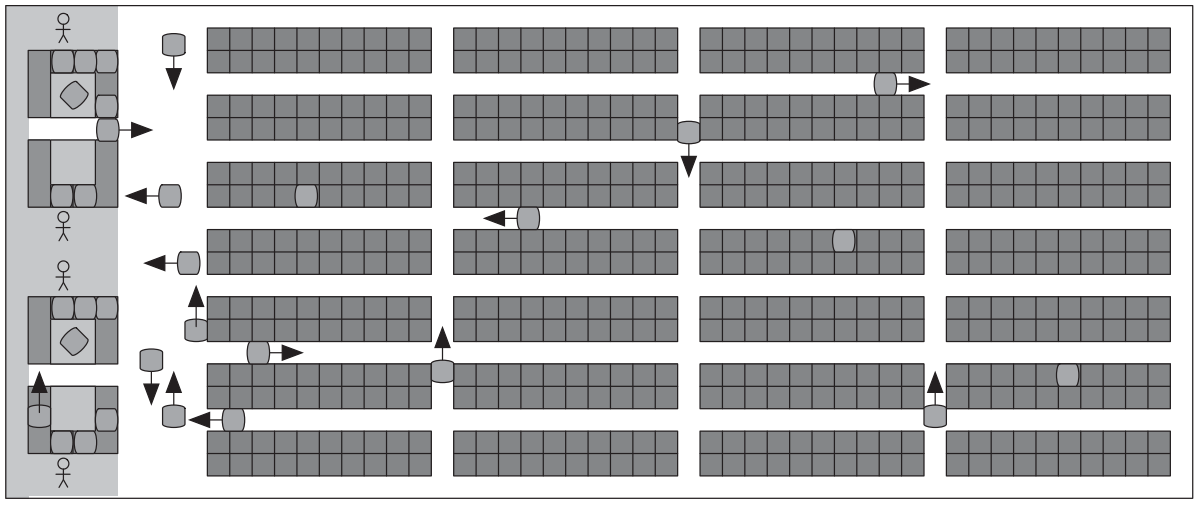
\includegraphics[width=0.9\textwidth]{graphics/kivasystemlayout}
	\caption{A Small Region of a Kiva Layout (\cite{wurman2008coordinating}). Picking stations located on the left and storage pods laid out in rows.}
	\label{kivalayout1}
\end{figure}

\cite{wilt2014spatially} looked at identifying zones by areas which are bottlenecks and assigning a controller, for that zone which manages any agents who need to travel through the bottleneck. Inspired by this and assuming pickup stations, we plan to split the warehouse into two halves and introduce an intermediate zone (See Fig \ref{kivalayout2}). Delivering pods which are situated in the far zone is a two step process:
\begin{compactenum}
	\item Units in the far zone move pods to the intermediate zone instead of a pickup station
	\item Units in the delivery zone will pickup pods in the intermediate zone
\end{compactenum}
\noindent These zones will have their own controller which handles any agents within the zone and tells them what behaviour should occur.

\begin{figure}[h]
	\centering
	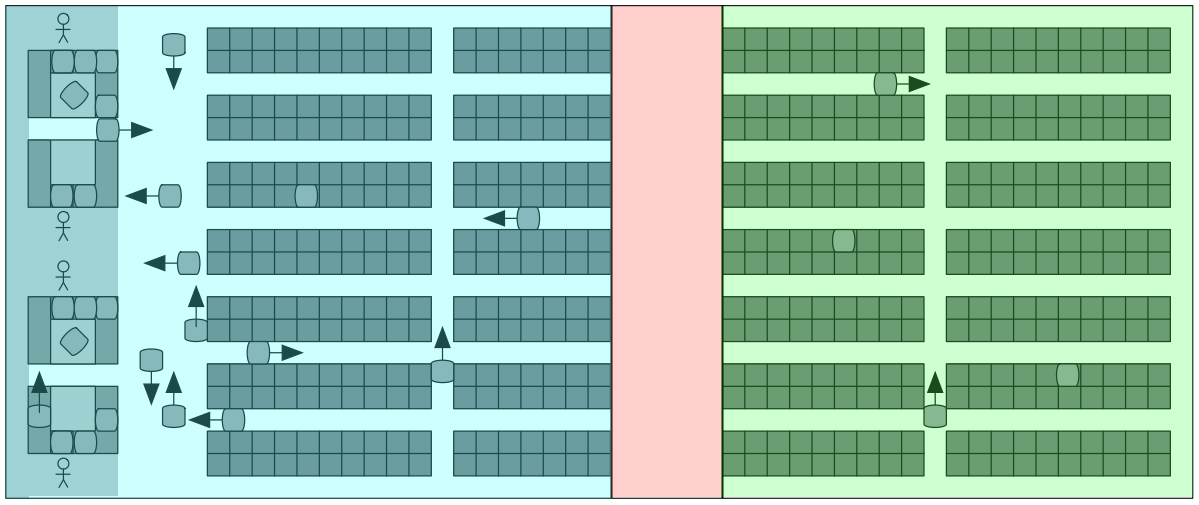
\includegraphics[width=0.9\textwidth]{graphics/kivasystemlayout_adjusted}
	\caption{Intermediate zone in red, delivery zone in blue and far zone in green}
	\label{kivalayout2}
\end{figure}

\subsection{Order processing}
\label{orderprocessing}
This problem is described in detail in Section \ref{background}. Reiterating the main points of order processing:

\begin{compactitem}
	\item A product distribution around the warehouse
	\item Smart sequencing of incoming orders according to the product distribution
\end{compactitem}

\noindent This is important to consider as determining the order process is dependent on the warehouse layout (Section \ref{warehouselayout}). We expect that an optimized order processing sequence will decrease the effects of having an inefficient warehouse layout. Here we may take inspiration from Robin-hood hashing or try implementing the optimizations described in \cite{boysen2017parts}.

\subsection{Allowing for movement underneath storage pods}
\label{beneathpods}
As drive units are capable of moving underneath pods when carrying them, this means that with small adjustments to the dimensions of storage pods it is possible to allow drive units to maneuver underneath the pods. With this the only obstacles in the environment are other drive units. Similar to order processing, this is important as it would greatly impact how we look at defining the warehouse layout.

\subsection{Timetable/plan}
\textbf{HALF DONE}
\begin{center}
{\footnotesize
\begin{tabular}{ c p{12cm} }
\multicolumn{2}{l}{\textbf{Semester 1}} \\
\hline \multicolumn{1}{c}{Week(s)} & \multicolumn{1}{c}{Plan} \\
\hline 7  & Create warehouse simulation with simple A* pathfinding \\
\hline 8-9  & Add multiple agents to the simulation using with Cooperative A* and moving between pickup stations \\
\hline 11 & Implement an order sequencer assigning generating an inflow of products to be retrieved \\
\hline 12 & Focus on Interim Presentation \\
\hline 13 & Focus on Literature Review \\
\hline 14 & Focus on Examinations \\
\hline Holidays & Look at the effects of warehouse layout and an intermediate dropping zone \\
\hline
\end{tabular}
}

{\footnotesize
\vspace{0.5cm}
\begin{tabular}{ c p{12cm} }
\multicolumn{2}{l}{\textbf{Semester 2}} \\
\hline \multicolumn{1}{c}{Week(s)} & \multicolumn{1}{c}{Plan} \\
\hline 1-3 & Implement Path Oracle with Compressed Path Databases \\
\hline 2-5 & Implement an optimized order processing method (\ref{orderprocessing}) \\
\hline 6-7 & Implement ability to move under pods (\ref{beneathpods}) \\
\hline 7-12 & Improve and analyze results, any extra time to explore any interesting findings more deeply \\
\hline 12 & Finish first draft of Final Thesis \\
\hline 13-15 & Focus on Final Presentation and Thesis \\
\hline
\end{tabular}
}
\end{center}

Weeks 7-15 in (semester 2) are not heavily populated as we will likely come across interesting areas while researching which we may decide to look at.

\section{Expected Outcomes}
Overall we aim to provide two major insights:

We suspect that these adjustments will reduce the number of conflicts in the MAPF problem hence allowing for a better bounded suboptimal solution to be found. Regardless of results, we expect to be able to better understand the explored properties described in Section \ref{Research} and their effect on Kiva systems.

Additionally we hope to deliver an improved MAPF solution utilizing a pre-computed path oracle and a simulation showcasing its usage in a Kiva system.

\bibliographystyle{dcu}
\bibliography{bibliography}


\end{document}
